% !TeX program = lualatex
\documentclass[
	english, % main language as globale option
	%logofile=example-image, % in case you are missing the logo files
	design=2023, % new slide design - will be default after official release
	]{tudabeamer}
	
\usepackage[main=english]{babel}

% Der folgende Block ist nur bei pdfTeX auf Versionen vor April 2018 notwendig
\usepackage{iftex}
\ifPDFTeX
\usepackage[utf8]{inputenc}%kompatibilität mit TeX Versionen vor April 2018
\fi
\usepackage{float}

\usepackage{graphicx}
\usepackage{amsmath}
\usepackage{amssymb}
\usepackage{pdfpages}
\usepackage[justification=centering]{caption}
\usepackage{subcaption}
\captionsetup[figure]{labelformat=empty}
\captionsetup[subfigure]{labelformat=empty}
\usepackage{animate}

\usepackage{amsmath}
\usepackage{amssymb}
\usepackage{bbold}
\usepackage{slashed}

\usepackage{animate}

\usepackage{xcolor}
\usepackage{url}
\newcommand{\Lagr}{\mathcal{L}}
\newcommand{\rectangle}{{\mathbin{\scalebox{2}[1]{$\square$}}}}

\newcommand{\sqbr}[1]{\left[#1\right]}
\newcommand{\rbr}[1]{\left(#1\right)}
\newcommand{\cbr}[1]{\left\{#1\right\}}

\newcommand{\pow}{^}

\usepackage{mathtools}
\DeclarePairedDelimiter\bra{\langle}{\rvert}
\DeclarePairedDelimiter\ket{\lvert}{\rangle}
\DeclarePairedDelimiterX\braket[2]{\langle}{\rangle}{#1\,\delimsize\vert\,\mathopen{}#2}

\DeclareMathOperator{\tr}{tr}
\DeclareUnicodeCharacter{2009}{\,}

\title[]{High-Precision Pressure
Measurement in Full Lattice
QCD for $N_f = 2+1$}
\subtitle{Abdelhamid Ettahri\\
Supervision: Guy D. Moore}
\author[]{Abdelhamid Ettahri}
\department{AG Moore}
\institute{Theoriezentrum Kernphysik}


%  titlegraphic will be placed behind the title
%\titlegraphic*{\includegraphics{example-image}}
\date{2026-04-01}

\begin{document}
\makeatletter
\setbeamertemplate{footline}{
  \leavevmode%
  \hbox{%
    \begin{beamercolorbox}[wd=.96\paperwidth,ht=2.5ex,dp=5ex,left]{author in head/foot}%
      \usebeamerfont{author in head/foot} {\fontsize{9pt}{9pt}\selectfont\hspace{1em}\phantom{\today}}
    \end{beamercolorbox}%
    
    \begin{beamercolorbox}[wd=.02\paperwidth,ht=2.5ex,dp=1ex,right]{date in head/foot}%
      {\fontsize{9pt}{9pt}\selectfont\insertframenumber{} \hspace{10em}}
    \end{beamercolorbox}%
  }%
  \vskip1pt%
}
\makeatother


\maketitle
\begin{frame}{Table of Contents}
\tableofcontents[columns=two, hidesubsections]
\end{frame}

% Redefine footline to change page number font size





\section{Motivation}
\begin{frame}
   \sectionpage
\end{frame}

\begin{frame}
\vspace{-0.5cm}
    \begin{figure}
        \centering
        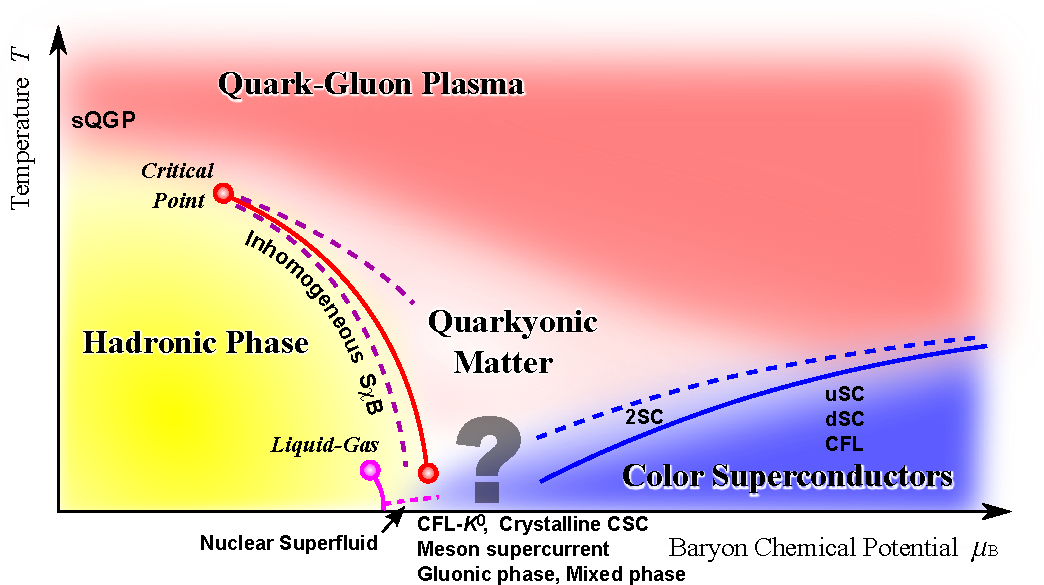
\includegraphics[width=0.8\linewidth]{images/phase.pdf}
    \end{figure}
\end{frame}




\section{Quantum Chromodynamics}
\begin{frame}
    \sectionpage
\end{frame}
\begin{frame}{QCD Lagrangian}
    \begin{align}
         \Lagr_{\text {QCD}}(\psi, \bar\psi, A)=\sum_f&\bar\psi^{(f)}(i\slashed \partial-m^{(f)})\psi^{(f)}\tag*{(free Dirac field)}\\
         &+\bar\psi^{(f)}\slashed A\psi^{(f)}\tag*{(Quark-Gluon interaction)}\\
         &-\frac{1}{2g^2}\tr\sqbr{G_{\mu\nu}^2}\tag*{(Gluodynamics)}
    \end{align}
     
\end{frame}


\begin{frame}{Pure Gauge Theory}
\begin{columns}
    \begin{column}{0.6\textwidth}
\begin{itemize}
    \item SU(3) local gauge invariance. $\slashed \partial\rightarrow \slashed D$
    \end{itemize}
    \begin{equation}
        D_\mu = \partial_\mu+igA^a_\mu t^a
    \end{equation}
    \begin{itemize}
    \item Field Strength tensor
    \end{itemize}
    \begin{align}
        G_{\mu\nu}&=\frac{i}{g}\sqbr{D_\mu,D_\nu}\\
        &=t^aG_{\mu\nu}^a=t^a\left(\partial_\mu A_\nu^a-\partial_\nu A_\mu^a+gA_\mu^b A_\nu^cf^{abc}\right)
    \end{align}
    \end{column}

     \begin{column}{0.4\textwidth}
     \vspace{-2cm}
     \centering
     \begin{figure}
         \centering
         \includegraphics[width=0.5\linewidth]{images/gluon_vertex.png}
         \caption{Gluon self-interaction}
     \end{figure}
    \end{column}
    \end{columns}
\end{frame}


\begin{frame}{Path Integral and Partition Function}
    \begin{itemize}
        \item The expectation value in a thermal setting at temperature $T$ is given by 
        \begin{equation}
            \langle \hat {\mathcal O}\rangle=\frac{\tr \hat A \hat \rho}{\tr \hat\rho},\qquad \hat\rho=\exp(-\beta_T\hat H),\qquad\beta_T=1/T
        \end{equation}
        \item Using the path integral formalism we may write
        \begin{equation}
            \langle\hat {\mathcal O}\rangle=\frac{\int_{\text{antiperiodic}}\mathcal D\bar\psi \mathcal D \psi\int _{\text{periodic}} \mathcal D A \exp\rbr{-\Lagr_E}\mathcal O (\bar\psi,\psi,A)}{\int_{\text{antiperiodic}}\mathcal D\bar\psi \mathcal D \psi\int _{\text{periodic}} \mathcal D A \exp\rbr{-\Lagr_E}}
        \end{equation}
        with $\tr \hat\rho =Z$ being nothing but the partition function.
    \end{itemize}
\end{frame}




\section{Lattice QCD}
\begin{frame}


\vspace{-1cm}
\begin{figure}
        \centering
        \includegraphics[width=0.5\linewidth]{images/lattice.png}
    \end{figure}

 \sectionpage
   
\end{frame}

\begin{frame}{Gauge invariance and Link Variables}
    \textbf{Continuum: }
    \begin{itemize}
        \item Introduce gauge fields $A_\mu$ to get a covariant derivative.
        \item Derivative compares infinitesimal separated points $\Rightarrow$ need elements of the Lie algebra
    \end{itemize}
    \textbf{Lattice:}
    \begin{itemize}
        \item Space-time is discretized $\Rightarrow$ points have finite separation
        \item Define Link variables as elements of the Lie Group $U_\mu(n)=\exp(iaA_\mu(n))$
    \end{itemize}
    \begin{figure}
        \centering
        \includegraphics[width=0.8\linewidth]{images/linkVariable.png}
    \end{figure}
\end{frame}

\begin{frame}{Wilson Gauge Action}
\begin{columns}
    \begin{column}{0.65\textwidth}
\begin{itemize}
        \item Closed loops of link variables can be used to construct a lattice version of the Gauge Action, such as the plaquette
        \begin{align*}
            U_{\mu\nu}(n)&=U_\mu(n)U_\nu(n+\hat\mu)U_{-\mu}(n+\hat\mu+\hat\nu)U_{-\nu}(n+\hat\nu)\\
            &=\exp(ia^2G_{\mu\nu}(n)+\mathcal{O}(a^3)).
        \end{align*}
        \item The Wilson Gauge action is now given by 
        \begin{equation*}
            S_G[U]=\frac{\beta}{3}\sum_{n\in\Lambda}\sum_{\mu<\nu}\text{Re tr}\sqbr{\mathbb1-U_{\mu\nu}(n)}.
        \end{equation*}
        with $\beta=6/g\pow2$.
    \end{itemize}
    \end{column}

    \begin{column}{0.35\textwidth}
        \begin{figure}
            \centering
            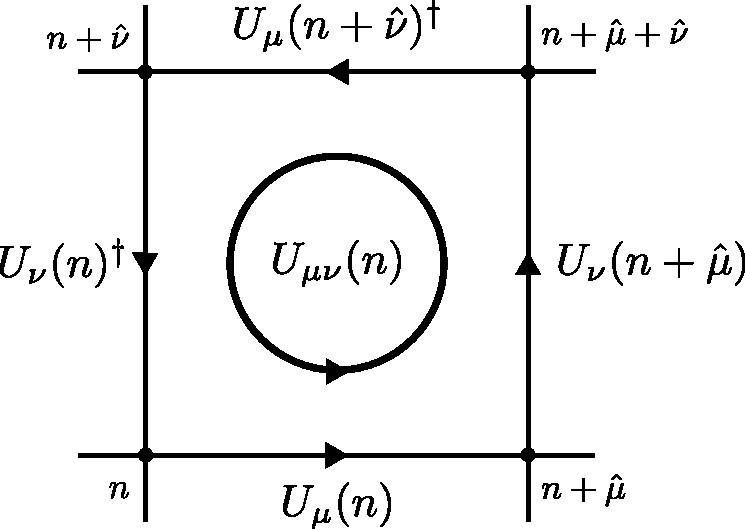
\includegraphics[width=\linewidth]{images/plaquette.pdf}
        \end{figure}
    \end{column}

    \end{columns}
\end{frame}

\begin{frame}{Lüscher-Weisz action}
    \begin{columns}
        \begin{column}{0.65\textwidth}
            \begin{itemize}
        \item Following the Symanzik improvement program Lüscher and Weisz decided to add further loops in the action.
        \begin{equation*}
    S_{G,LW}=\frac{\beta}{3}\cbr{\frac{5}{3}\sum_\square\text{tr } \sqbr{\mathbb 1-U(\square)}-\frac{1}{12}\sum_\rectangle \text{tr}\sqbr{\mathbb 1-U(\rectangle)}}.
\end{equation*}
\item The Wilson gauge action has an $\mathcal{O}(a^2)$ error, which is canceled in the improved action.
\end{itemize}
        \end{column}  
        \begin{column}{0.35\textwidth}
            \begin{figure}
                \centering
                \includegraphics[width=\linewidth]{images/luescherLoops.png}
            \end{figure}
        \end{column}
    \end{columns}
    
\end{frame}

\begin{frame}{Fermion Action and Doublers}
    \begin{itemize}
        \item Discretizing the derivative we may define the naive fermion action
        \begin{equation}
             S_{\text{F,naive}}=a^4\sum_{n\in\Lambda}\bar\psi(n) \rbr{\gamma_\mu\frac{U_\mu(n)\psi(n+\hat\mu)-U_{-\mu}(n)\psi(n-\hat\mu)}{2a}+m\psi(n)}.
        \end{equation}
        \item The corresponding propagator in momentum space
        \begin{equation}
            \tilde D(p)=m\mathbb 1 +\frac{i}{a}\sum_\mu\gamma_\mu\sin(p_\mu a)
        \end{equation}
        16 zeros instead of one for $m=0$ leading to the Fermion Doublers.
    \end{itemize}
\end{frame}

\begin{frame}{Chiral Symmetry}
    \begin{itemize}
        \item Chiral symmetry (and its spontaneous breaking) explains important features of QCD, such as low pion masses.
        \item For massless quarks the $\Lagr_{QCD}$ is invariant under chiral transformations
        \begin{equation}
            \psi\rightarrow e^{i\alpha\gamma_5}\psi,\qquad \bar\psi\rightarrow\bar\psi e^{i\alpha\gamma_5},\qquad \gamma_5=\gamma_1\gamma_2\gamma_3\gamma_4
        \end{equation}
        \item Wilson solved the Fermion Doubler problem by adding a term, but it breaks chiral symmetry
        \item \textbf{Nielsen-Ninomiya Theorem}: On the lattice we cannot have chiral symmetry and no Fermion Doublers.
    \end{itemize}
\end{frame}

\begin{frame}{Staggered Fermions}
    \begin{itemize}
        \item Perform a position dependent rotation in Dirac space
        \begin{equation}
        \psi(n)=\gamma_1^{n_1}\gamma_2^{n_2}\gamma_3^{n_3}\gamma_4^{n_4}\psi(n)', \quad \bar\psi(n)=\bar\psi(n)'\gamma_4^{n_4}\gamma_3^{n_3}\gamma_2^{n_2}\gamma_1^{n_1}
        \end{equation}
        \item Using the commutation relation of the gamma matrices we find thea sign function such that
        \begin{equation}
             \bar\psi(n)\gamma_\mu\psi(n\pm\hat\mu)= \eta_\mu(n)\bar\psi(n)'\psi(n\pm\hat\mu)'.
        \end{equation}
        \item The transformation diagonalizes the dirac operator in the spinor space and we can decide to only keep one component, which reduces the number of doublers from 16 to 4 (tastes).
        \item The Highly Improved Staggered Quark (HISQ) action reduces errors by smearing the link variables and adding further terms. 
    \end{itemize}
\end{frame}



\section{Thermodynamics}
\begin{frame}
    \sectionpage
\end{frame}
\begin{frame}{Pressure from the Partition Function}
    \begin{itemize}
        \item The Partition Function can be simplified to
        \begin{equation}
             Z(\beta,m)=\int \mathcal DU \det[\slashed D+m]\exp\rbr{-\beta S_G[U]}
        \end{equation}
        \item In the thermodynamic limit the pressure is given by
        \begin{equation}
            P=\frac{T}{V}\ln Z
        \end{equation}
        which can be used to calculate the trace anomaly, the energy and entropy density and also the speed of sound
        \begin{equation}
            I=3P-\epsilon=-T^5\frac{\partial}{\partial T}\frac{P(T)}{T^4},\qquad  s=\frac{P+\epsilon}{T},\quad c_s^2=\frac{dP}{d\epsilon}.
        \end{equation}
    \end{itemize}
\end{frame}

\begin{frame}{Integral Method I}
    \begin{itemize}
        \item Lattice calculation can be used to calculate expectation values but not the partition function itself.
        \item Using the integral method we can rewrite the pressure formula in terms of derivatives of $Z$.
        \begin{align}
            P(\beta, m)-P(\beta_0,m_0)&= \int_{\lambda_0}^{\lambda}d\lambda'\frac{\partial \ln Z}{\partial \lambda'}\\
            &=\int_{(\beta_0,m_0)}^{(\beta,m)}\rbr{d\beta'\frac{\partial\ln Z}{\partial \beta'}+dm'\frac{\partial \ln Z}{\partial m'}}.
        \end{align}
    \end{itemize}
\end{frame}

\begin{frame}{Integral Method II}
    \begin{itemize}
        \item The derivatives reduce to expectation values
        \begin{align}
            \frac{\partial \ln Z}{\partial \beta}&=\frac{1}{Z}\int \mathcal DU \det[\slashed D+m]\exp\rbr{-\beta S_G[U]} (-S_G[U])=\langle-S_G\rangle.\\
            \frac{\partial \ln Z}{\partial m}&=\frac{1}{Z}\int \mathcal DU \det[\slashed D+m]\exp\rbr{-\beta S_G[U]} \tr\frac{1}{\slashed D+m}
     =\left\langle\tr\frac{1}{\slashed D+m}\right\rangle=\langle\bar\psi\psi\rangle.
        \end{align}
        \item The Pressure is the given by
        \begin{equation}
            P(\beta, m)-P(\beta_0,m_0)=\int_{(\beta_0,m_0)}^{(\beta,m)}\rbr{d\beta'\langle-S_G\rangle+dm'\langle\bar\psi\psi\rangle}. 
        \end{equation}
    \end{itemize}
\end{frame}




\section{Measuring Process}

\begin{frame}
\sectionpage
\end{frame}

\begin{frame}{Monte Carlo Integration}
\begin{columns}
    \begin{column}{0.6\textwidth}
         \begin{itemize}
        \item The expectation value is given by an infinite dimensional integral
        \begin{align*}
    \langle \mathcal O\rangle=\frac{1}{Z} \int\mathcal D[U]\exp\rbr{-S_G[U]}\mathcal O[U]
\end{align*}
    \item Instead we generate $N$ configurations of $U$ according to the correct probability distribution and compute
    \begin{equation}
         \frac{1}{N}\sum_{n=1}^NO[U_n].
    \end{equation}
    \end{itemize}
    \end{column}
    \begin{column}{0.4\textwidth}
        \vspace{-1.5cm}
        \begin{figure}
            \centering
            \includegraphics[width=0.8\linewidth]{images/monteCarlo.png}
            \caption{https://www.geeksforgeeks.org/artificial-intelligence/what-is-monte-carlo-simulation/}
        \end{figure}
    \end{column}
\end{columns}
   
\end{frame}

\begin{frame}{Markov Chains and Metropolis Algorithm}
    \begin{columns}
    \begin{column}{0.7\textwidth}
         \begin{itemize}
        \item Generate configurations via Markov chain satisfying ergodicity.
        \end{itemize}
        \textbf{Metropolis:}
        \begin{itemize}
        \item 1: Choose candidate configuration $U'$ according to a priori selection probability $T_0(U'|U)$
        \item 2: Accept $U'$ with probability 
        \begin{equation*}
            T_A(U'|U)=\min\rbr{1,\frac{T_0(U|U')\exp(-S[U'])}{T_0(U'|U)\exp(-S[U])}}=\min(1,\exp(-\Delta S))
        \end{equation*}.
    \end{itemize}
    \end{column}
    \begin{column}{0.3\textwidth}
        \begin{figure}
            \centering
            \includegraphics[width=0.9\linewidth]{images/markov.png}
            \caption{Sketch of a Markov chain}
        \end{figure}
    \end{column}
\end{columns}
\end{frame}

\begin{frame}{Heat Bath and Overrelaxation}
    \begin{itemize}
        \item Both Algorithms generate configurations in a way skipping the accept/reject step
        \item They are actually defined for $SU(2)$ matrices exploiting that a sum of two $SU(2)$ matrices is just a scaled $SU(2)$ matrix
        \end{itemize}
        \textbf{Heat Bath:}
        \begin{itemize}
        \item Change one link variable at a time exploiting the locality of the gauge action.
        \item Disadvantage: Thermalization is time-consuming.
    \end{itemize}
    \textbf{Overrelaxation:}
    \begin{itemize}
        \item Change the configuration globally without changing the action
        \item Disadvantage: Not ergodic since we stay in subspace of constant action.
    \end{itemize}
\end{frame}

\begin{frame}{Fermion determinant}
    \begin{itemize}
    \item In pure glue and quenched QCD we ignore the fermion determinant completely
        \item When including dynamical fermions, the fermion determinant has to be included as a weight factor
        \item Problem: Highly non-local expression
        \item Instead we work with pseudo fermions, formulating fermions via complex bosonic fields using
        \begin{equation}
             \det\sqbr{DD^\dagger}=\pi^{-N}\int\mathcal D\phi_I\mathcal{D}\phi_R\exp\rbr{-\phi^\dagger\rbr{DD^\dagger}^{-1}\phi}
        \end{equation}
    \end{itemize}
\end{frame}

\begin{frame}{Hybrid Monte Carlo}
    \begin{itemize}
        \item The unquenched theory is expensive $\Rightarrow$ Have to change the action globally with high acceptance rate
        \item Goal: Try not to change the action 
        \item Rough idea: Simulate the dynamics of classical particles that do not change the Hamiltonian
        \begin{equation}
            H[Q,P]=\frac{1}{2}P^2+S[Q]
        \end{equation}
        by solving the Hamilton equations
        \begin{equation}
            \dot P =-\frac{\partial H}{\partial Q},\qquad \dot Q=P.
        \end{equation}
    \end{itemize}
\end{frame}

\section{Outlook}
\begin{frame}
\sectionpage
\end{frame}
\begin{frame}{Setup}
    \textbf{Lattice Action: HISQ/tree}
    \begin{itemize}
        \item Gauge Action: Lüscher-Weisz Action with parameters $\beta_\square$ and $\beta_\rectangle$
        \item Fermion Action: Highly Improved Staggered Fermion Action with parameters $m_u=m_d$ and $m_s$ ($N_f=2+1$)
    \end{itemize}
    \begin{table}[h]
\centering
\begin{tabular}{c c c c c c}
\hline
$\beta$ & $m_l$ & $m_s$ & $n_\tau$ & $T$ (MeV) \\
\hline
7.373 & 0.00125 & 0.0250 & 8  & 409.7 \\
7.596 & 0.00101 & 0.0202 & 10 & 400.0 \\
7.825 & 0.00082 & 0.0164 & 12 & 407.4 \\
\hline
\end{tabular}
\end{table}
        
\end{frame}

\begin{frame}{Plan}
    \begin{columns}
        \begin{column}{0.6\textwidth}
           \begin{enumerate}
               \item Pure Glue
               \begin{itemize}
                   \item Move from zero coupling to ''above'' the point of interest
                   \item Do not cross the phase transition
                   \item Either stay in Lüscher-Weisz or move to Wilson action 
               \end{itemize}
               \item Full QCD
               \begin{itemize}
                   \item Start with infinitely heavy quarks and go to lighter masses while keeping all quark masses the same
                   \item Move to correct quark masses
               \end{itemize}
           \end{enumerate}
        \end{column}
        \begin{column}{0.4\textwidth}
            \begin{figure}
                \centering
                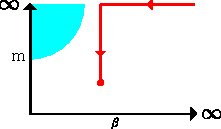
\includegraphics[width=0.9\linewidth]{images/path.pdf}
            \end{figure}
        \end{column}
    \end{columns}
\end{frame}

\begin{frame}[allowframebreaks]{References}
\footnotesize
\nocite{*}
\bibliographystyle{plain}
\bibliography{references}
\end{frame}

\end{document}